\documentclass[sigconf]{acmart}

\usepackage{booktabs} % For formal tables
\usepackage{listings}

\lstset{
  basicstyle=\ttfamily\small,
  columns=fullflexible,
  breaklines=true,
}

\title{Optimizing Zero-Shot Model Compression Pipelines: A Progress Report}
\author{Henry Morgan}
\affiliation{%
  \institution{University of Washington Bothell}
  \country{USA}
}
\email{hdmorgan@uw.edu}

\begin{abstract}
Modern deep learning models are often too large and computationally expensive for deployment on resource-constrained edge devices. Model compression techniques such as quantization, pruning, and knowledge distillation are essential for optimizing these models. This project systematically explores the effects of combining these techniques in a zero-shot (data-free) setting. We have implemented a flexible pipeline that allows for the sequential application of various compression methods and evaluates their impact on model size, sparsity, and latency. This report details the progress made in implementing these compression techniques, the pipeline infrastructure, and initial experimental results. We also outline the plan for the final paper, which will involve more extensive experiments and analysis.
\end{abstract}

\begin{document}
\maketitle

\section{Introduction}
The increasing size and complexity of state-of-the-art deep learning models present significant challenges for their deployment on edge devices with limited computational power and memory. Model compression aims to reduce the size and inference latency of these models while preserving their predictive accuracy. This project focuses on zero-shot compression techniques, which are particularly valuable as they do not require access to the original training data.

Our primary goal is to understand the interactions between different compression methods and to identify optimal orderings for their application. We have developed a modular framework in Python using PyTorch to construct and evaluate various compression pipelines.

\section{Project Progress}

\subsection{System Design and Implementation}
We have designed and implemented a \texttt{CompressionPipeline} that orchestrates the application of multiple compression techniques. The core components of our system are:

\begin{itemize}
    \item \textbf{BaseCompressor Interface:} An abstract base class that defines a common interface for all compression techniques. Each compressor implements a \texttt{compress} method that takes a model and returns a compressed model along with metadata.
    \item \textbf{Compression Techniques:} We have implemented the following zero-shot compression techniques:
    \begin{itemize}
        \item \textbf{Quantization:} \texttt{DynamicQuantizer} and \texttt{StaticQuantizer} to reduce model precision to INT8.
        \item \textbf{Pruning:} \texttt{MagnitudePruner} for unstructured pruning and \texttt{StructuredPruner} for structured pruning of weights.
        \item \textbf{Knowledge Distillation:} \texttt{ZeroShotDistiller} that synthesizes pseudo-inputs from the teacher model's batch normalization statistics.
    \end{itemize}

\end{itemize}

The overall workflow is managed by the \texttt{run\_experiment.py} script, which defines and executes different pipeline configurations, collects metrics, and presents a comparative summary.

\subsection{Initial Experiments and Results}
We conducted an initial set of experiments to compare different orderings of dynamic quantization and magnitude pruning. The results are summarized in Table~\ref{tab:results}. The key trade-offs between model size and inference latency are visualized in Figure~\ref{fig:size} and Figure~\ref{fig:latency}.

\begin{table}[h]
  \caption{Experiment Results Summary}
  \label{tab:results}
  \begin{tabular}{lccc}
    \toprule
    Pipeline & Size (MB) & Sparsity (\%) & Latency (ms)\\
    \midrule
    Baseline (no compression)                     & 0.39 & 0.00 & 0.06 \\
    Dynamic Quantization only                     & 0.10 & 0.00 & 0.33 \\
    Magnitude Pruning (50\%) only                 & 0.39 & 50.00 & 0.07 \\
    Structured Pruning (30\%) only                & 0.39 & 30.08 & 0.06 \\
    Prune → Quantize                            & 0.10 & 0.00 & 0.31 \\
    Quantize → Prune                            & 0.10 & 0.00 & 0.24 \\
    Structured Prune → Magnitude Prune → Quantize & 0.10 & 0.00 & 0.30 \\
    \bottomrule
  \end{tabular}
\end{table}

\begin{figure}[h]
  \centering
  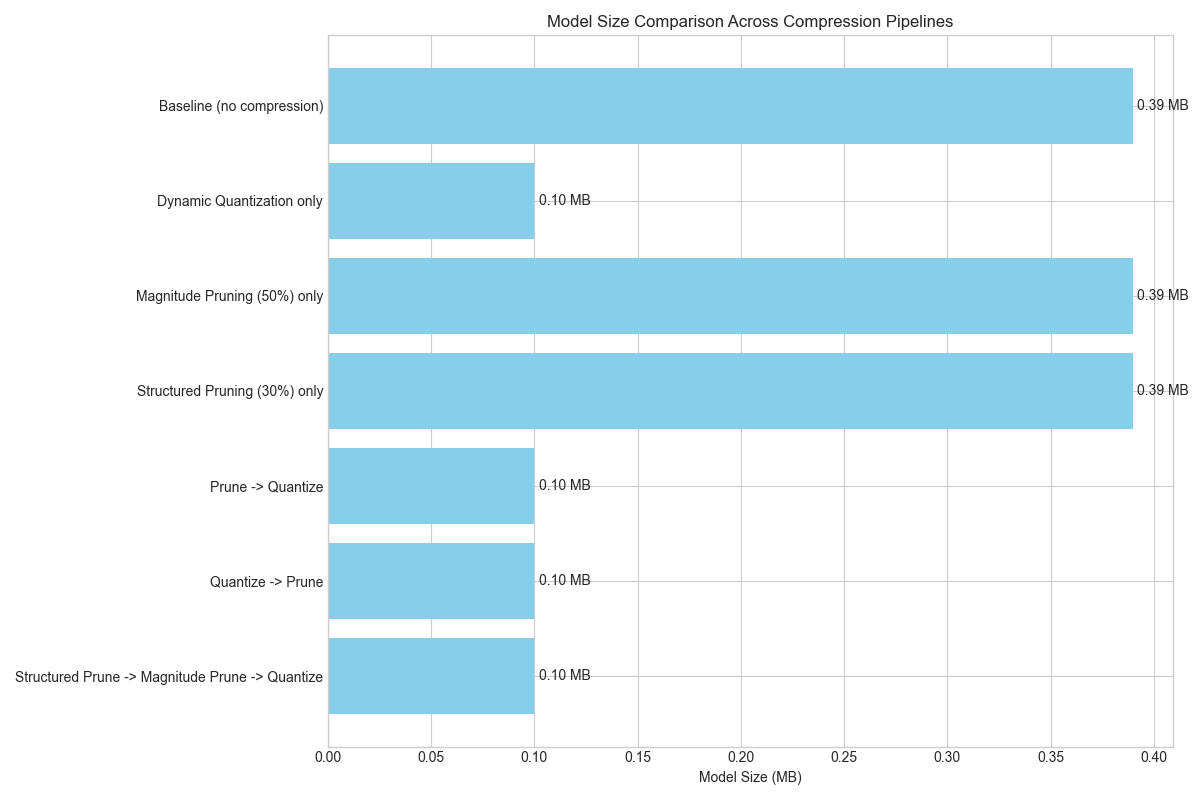
\includegraphics[width=\linewidth]{../results/model_size_comparison.png}
  \caption{Model Size Comparison Across Compression Pipelines.}
  \label{fig:size}
\end{figure}

\begin{figure}[h]
  \centering
  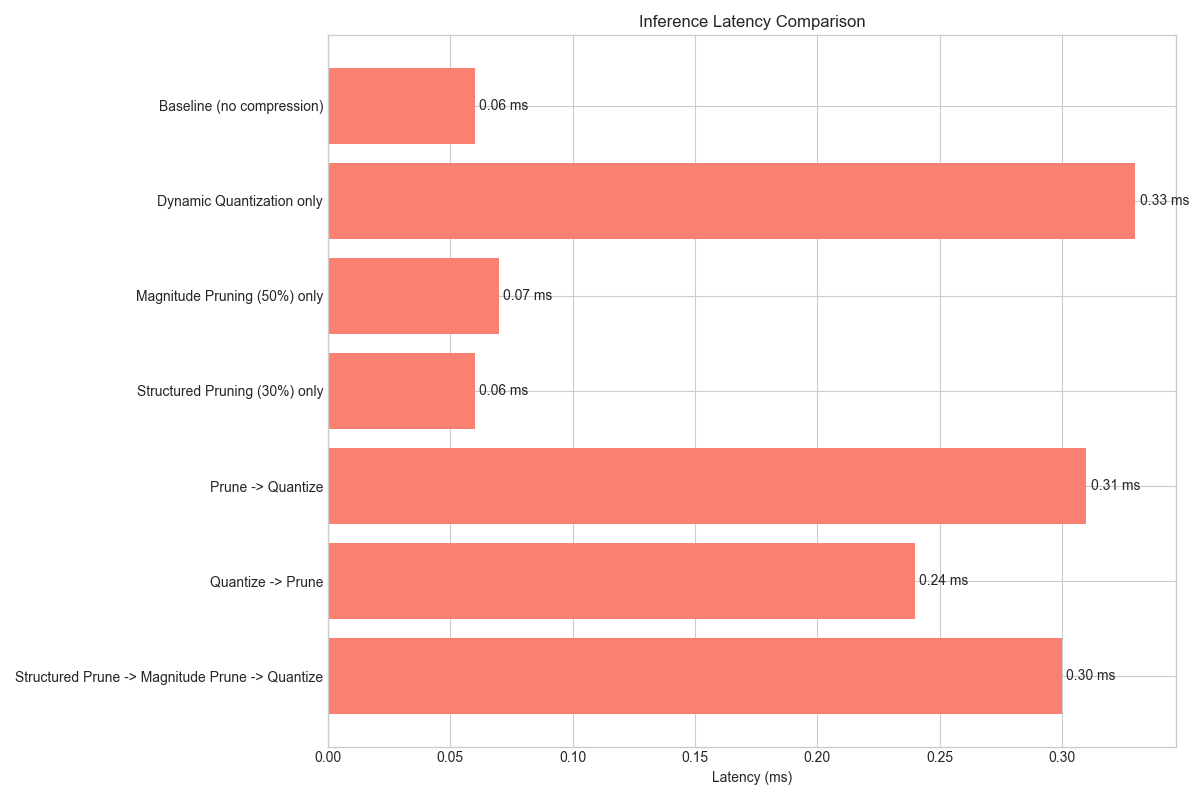
\includegraphics[width=\linewidth]{../results/latency_comparison.png}
  \caption{Inference Latency Comparison Across Compression Pipelines.}
  \label{fig:latency}
\end{figure}

From these initial results, we observe that quantization is highly effective at reducing model size, but it can introduce latency overhead. Pruning, especially structured pruning, shows promise in reducing model complexity without significantly impacting latency in this zero-shot setting. The combination and ordering of these techniques lead to interesting trade-offs that warrant further investigation.

\subsection{Unit Testing}
We have implemented a comprehensive suite of unit tests using \texttt{pytest} to ensure the correctness of our compression components and evaluation metrics. All 20 tests are currently passing, confirming the reliability of our implementation.

\begin{lstlisting}
============================= test session starts ==============================
...
============================= 20 passed in 2.80s ===============================
\end{lstlisting}

\section{Plan for Final Paper}
Our plan for the final paper includes the following steps:

\begin{enumerate}
    \item \textbf{Literature Review:} Conduct a thorough review of existing literature on model compression and pipeline optimization. Recent work has shown the effectiveness of combining Neural Architecture Search (NAS) with Knowledge Distillation (KD) to automatically discover optimal student architectures that balance performance and efficiency. This ``KD-NAS'' approach, as detailed by Trivedi et al. (2023) \cite{trivedi2023neural}, moves beyond manually selecting student models and instead searches a predefined space of architectures to find one best suited for distillation from a given teacher. This is a promising direction for automating and improving the compression process. Vilar Dantas et al. (2024) \cite{vilar2024comprehensive} provide a comprehensive review of model compression techniques, which will serve as a foundational reference for our work.
    \item \textbf{Expand Experiments:}
    \begin{itemize}
        \item Incorporate \texttt{StaticQuantizer} and \texttt{ZeroShotDistiller} into the experimental pipeline.
        \item Apply the compression pipelines to a pre-trained model from \texttt{torchvision} (e.g., ResNet-18) to evaluate performance on a real-world task.
        \item Measure the impact on model accuracy on a validation dataset (e.g., CIFAR-10).
    \end{itemize}
    \item \textbf{Analyze and Visualize Results:} Create plots and tables to clearly present the trade-offs between model size, latency, and accuracy for different compression strategies.
    \item \textbf{Future Work -- NAS Integration:} As an extension, we will explore integrating a NAS component into our pipeline. This would involve defining a search space of possible student architectures and using a search strategy (e.g., reinforcement learning) to find an optimal student for our \texttt{ZeroShotDistiller}, automating a key part of the pipeline design, as inspired by the work of Merler et al. (2025) \cite{merler2025neural}.
    \item \textbf{Write Final Paper:} Structure the final paper with a comprehensive literature review, detailed methodology, thorough experimental results, and a concluding discussion on the findings.
\end{enumerate}

\bibliographystyle{ACM-Reference-Format}
\bibliography{references}

\end{document}
